\documentclass[14pt]{beamer}
\usepackage[utf8]{inputenc}
\usepackage[T1]{fontenc}
\usepackage{multirow,tabularx}
\usepackage{amsmath}
\usepackage{pgf}

\usetheme{Antibes}
\usecolortheme{orchid}
\usefonttheme{serif}

\title{Prezentacja o Sawannie}
\author{Tomasz Wnuk}
\institute{Uniwersytet Marii Curie-Skłodowskiej}
\date{Styczeń 2022}

\begin{document}

\maketitle
\section{Definicje}

\begin{frame}{\color{black}{Co to jest sawanna?}}
    \begin{block}{\color{red}{O Sawannie}}
        \small  \textit{Sawanna to formacja trawiasta występująca w strefie międzyzwrotnikowej
        \small  na obszarach o suchym i gorącym klimacie z wyraźnie zaznaczoną
        \small  sezonowością. Sawanna złożona jest z wysokich traw oraz pojedynczych drzew i krzewów.}
    \end{block}
    \begin{figure}
        \centering
        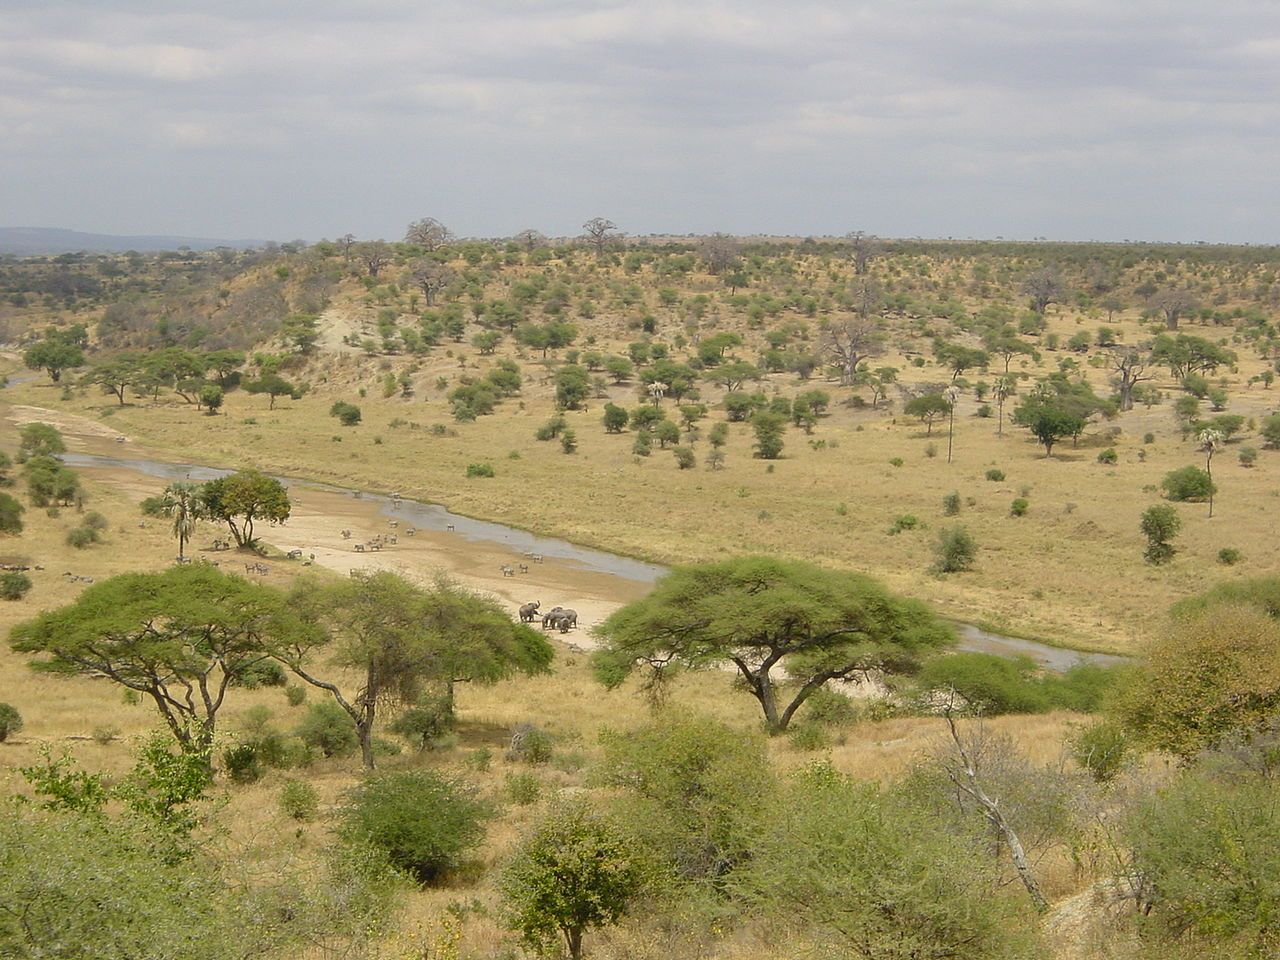
\includegraphics[scale=0.1]{Sawanna_w_tanzanii.jpg}
        \caption{Sawanna w Tanzanii}
        \label{fig:my_label}
    \end{figure}
\end{frame}

\subsection{Flora i fauna}

\begin{frame}{\color{black}{Roślinność}}
    \tiny   \uppercase{Warunki klimatyczne obszarów}, na których występuje sawanna (pora sucha i pora deszczowa) wymuszają istnienie specyficznej roślinności. Największe powierzchnie zajmują trawy dobrze przystosowane do przetrwania pory suchej. Ich źdźbła rosną przy podstawie, a nie na wierzchołku. Dzięki temu trawa wyskubywana z góry przez zwierzęta może rosnąć dalej. Niektóre z traw sawanny (np. trawa słoniowa) osiągają imponujące rozmiary, dorastając nawet do 5 metrów wysokości.
    \tiny   \textbf{Krzewy rosnące na sawannie często gromadzą wodę w tkankach łodyg lub liści.}  Wiele z nich, np. aloes czy wilczomlecz, wykształca kolce do ochrony przed roślinożercami. Innym sposobem ochrony przed utratą cennej wody jest przekształcenie liści w suche i twarde twory przypominające długie igły sosny. Przykładem takiego krzewu (a czasem drzewa) jest australijska kazuaryna.
    \tiny   \emph{Drzewa są na sawannie nieliczne, gdyż stada roślinożerców zadeptują ich siewki lub zjadają je, zanim zdążą urosnąć.} Jeśli jednak im się to uda, osiągają często ogromne rozmiary. Dzięki rozmiarom swych korzeni, sięgających kilka metrów w głąb i wiele metrów wszerz, mają największe możliwości czerpania wody z głębszych warstw. Ale w końcu im także w porze suchej brakuje wody. Niektóre drzewa sawanny w porze deszczowej gromadzą wodę w pniach, np. baobaby. Inne, jak eukaliptusy, wytwarzają odporne na suszę skórzaste liście, ustawiające się brzegiem do słońca. Jeszcze inne mają drobne liście i długie ciernie, jak akacje. Zdarza się, że gdy susza utrzymuje się przez długi czas, to drzewa zrzucają liście, by ograniczyć parowanie.
\end{frame}

\begin{frame}{\color{black}{Zdjęcia roślinności}}
    \begin{figure}
        \centering
        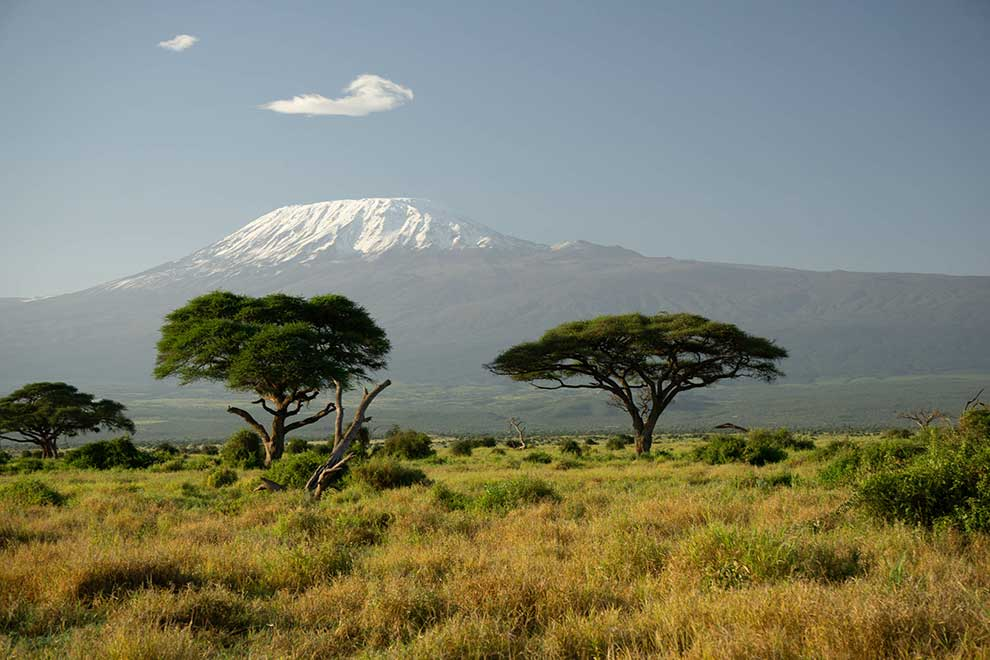
\includegraphics[scale = 0.25]{Sawanna1.jpg}
        \caption{Przykłady drzew i krzewów}
        \label{fig:my_label}
    \end{figure}
\end{frame}

\begin{frame}{\color{black}{Zwierzęta}}
    \tiny   \underline{Szybko rosnące w porze deszczowej trawy zapewniają ogromne ilości pożywienia dla zwierząt.} Dzięki temu na afrykańskich sawannach spotykamy duże ssaki roślinożerne: słonie, nosorożce, żyrafy i bawoły. W wielkich stadach wędrują po sawannie zebry i różne gatunki antylop. Na sawannach Ameryki Południowej nie ma tak wielkich stad i tak wielkich roślinożerców. Wśród ssaków kopytnych uwagę zwraca jeleń pampasowy. W sąsiedztwie rzek żyją tu największe gryzonie świata – kapibary, a ciekawostką są niespotykane na innych kontynentach mrówkojady czy pancerniki. W Australii największymi zwierzętami sawanny są kangury. W ostatnich latach pojawia się tam coraz więcej zdziczałych wielbłądów przywiezionych przez ludzi.
    \tiny   W ślad za roślinożercami podążają liczne drapieżniki. W Afryce wielkimi mięsożercami są m.in. lwy, lamparty oraz nieco lżejsze, ale bardzo szybkie gepardy. Mniejsze od nich są hieny, szakale i likaony, które zespołowo polują lub zadowalają się resztkami po uczcie większych drapieżników. Największymi drapieżnikami sawanny w Ameryce Południowej są jaguar i wilk grzywiasty, a w Australii dziki pies dingo.
    \tiny   Typowe dla sawanny są wielkie nielotne ptaki, jak afrykańskie strusie i ich nieco mniejsze odpowiedniki: nandu w Ameryce Południowej i emu w Australii. Wszędzie pojawiają się wielkie padlinożerne sępy. W Afryce charakterystycznym ptakiem sawanny jest marabut. Na sawannach wszystkich kontynentów żyje wiele gadów (szczególnie węży i jaszczurek) i niezliczone bezkręgowce (termity, mrówki, szarańczaki, pająki).
    \tiny   Sawanny są też miejscami zamieszkania ludzi, którzy zajmują się uprawą roli, chowem kóz, bydła i koni oraz polowaniem. To doskonałe miejsce na wypas ogromnych stad bydła.
\end{frame}

\begin{frame}{\color{black}{Zdjecie zebr na sawannie}}    
    \begin{figure}
        \centering
        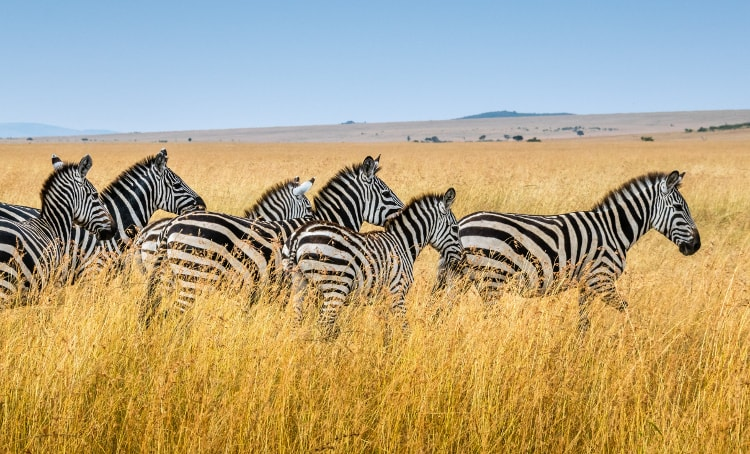
\includegraphics[scale = 0.4082]{Sawanna2.jpg}
        \label{fig:my_label}
    \end{figure}
\end{frame}

\begin{frame}{\color{black}{Ludzie na sawannie}}
    \tiny  Obecnie sawanny są zamieszkane, ale gospodarka ogranicza się do hodowli zwierząt i uprawy roli. Ważnym czynnikiem ekonomicznym stała się turystyka. Niegdyś do Afryki organizowano myśliwskie wyprawy – safari. Bogaci ludzie polowali na dzikie zwierzęta, by móc pochwalić się trofeami. W pałacach wieszano spreparowane głowy zwierząt, poroża, z kości słoniowej robiono ozdoby i leki. Doprowadziło to do ogromnego spadku liczebności dzikich zwierząt. Na szczęście w ostatnich latach udało się go zahamować. Teraz dla turystów organizuje się „bezkrwawe łowy” – safari, w czasie których zwierzęta można obserwować i fotografować w naturalnym środowisku w parkach i rezerwatach. Praca strażnika w parku narodowym lub przewodnika turystów stanowi znaczące źródło dochodu dla lokalnych społeczności.
\end{frame}

\begin{frame}{\color{black}{Tabela}}
    \begin{table}[]
        \centering
        \caption{Sample ANOVA table}
        \begin{tabular}{c c c c c} 
            \hline
            Stubhead & df & f & n & p \\ [0.5ex] 
            \hline
            & & \multicolumn{2}{c}{Spanning text} \\
            Row 1 & 1 & 0.67 & 0.55 & 0.41 \\
            Row 2 & 2 & 0.02 & 0.01 & 0.39 \\
            Row 3 & 3 & 0.15 & 0.33 & 0.34 \\
            Row 4 & 4 & 1.00 & 0.76 & 0.54 \\
            \hline
        \end{tabular}
    \end{table}
\end{frame}

\begin{frame}{\color{black}{Wzór}}
    \begin{displaymath}
        t \rightarrow t’ = \frac{1}{\sqrt{1-\frac{v^{2}}{c^{2}}}}(t-\frac{v}{c^{2}}x)
    \end{displaymath}
    \begin{displaymath}
        x \rightarrow x’ = \frac{1}{\sqrt{1-\frac{v^{2}}{c^{2}}}}(x-vt)
    \end{displaymath}
\end{frame}

\section{}

\begin{frame}{\color{black}{Dziękuję za uwagę}}
    Źródła:
    \begin{enumerate}
        \item Punkt pierwszy źródła:
            \begin{itemize}
                \item zpe.gov.pl
                \item rzucijedz.pl
                \item www.medianauka.pl
                \item pl.wikipedia.org
        \end{itemize}
        \item Punkt drugi
        \item Punkt trzeci
        \item Punkt czwarty
    \end{enumerate}
\end{frame}

\end{document}
